\documentclass{SCIS2023cn}

\usepackage{listings}

\begin{document}
	
\lstset{language=Java, 
	basicstyle=\ttfamily\small, 
	keywordstyle=\color{blue}\bfseries, 
	commentstyle=\color{red}, 
	stringstyle=\color{red}, 
	showstringspaces=false,
	breaklines=true,
	numbers=left,
	frame=single}

\ArticleType{课程总结}
\Year{2023}
\Vol{53}
\No{1}
\BeginPage{1}
\DOI{}
\ReceiveDate{}
\ReviseDate{}
\AcceptDate{}
\OnlineDate{}
\AuthorMark{}
\AuthorCitation{}
\enAuthorCitation{}

\title{My Perspective on Software Architecture}{引用的标题}

\entitle{My Perspective on Software Architecture}{Title for citation}

\author[1]{名字}{Name}{mail@smail.nju.edu.cn}

\address[1]{南京大学\ 匡亚明学院, 南京 210093}{Kuang Yaming Honors School, Nanjing University, Nanjing {\rm 210093}, China}

\abstract{作为控制软件复杂性、提高软件系统质量、支持软件开发和复用的重要手段之一,软件体系结构自提出以来,日益受到软件研究者和实践者的关注,并发展成为软件工程的一个重要的研究领域。系统的软件架构展示与整个系统结构和行为相关的设计决策。随着软件工程规模的扩大,算法相关的内容占比降低,如何设计良好的软件体系结构以维持软件系统的灵活性、高可用性和可维护性变得更加重要。本文是《软件体系结构》课程的课程总结,将介绍包括分层系统、MVC在内常见的软件架构,并分享笔者个人对软件架构的理解。}

\enabstract{As one of the important means to control software complexity, improve software system quality, support software development and reuse, software architecture has increasingly attracted the attention of software researchers and practitioners since its inception, and has developed into an important research field in software engineering. The software architecture of a system represents the design decisions related to overall system structure and behavior. With the expansion of software engineering scale, the proportion of algorithm related content has decreased. It has become more important to design a good software architecture to maintain the flexibility, high availability, and maintainability of software systems. This article is a course summary of the Software Architecture course, which will introduce common software architectures including layered systems and MVC, and share the author's personal understanding of software architecture.}

\keywords{软件体系结构, 软件工程, 敏捷开发,课程总结}
\enkeywords{software architecture, software engineering, agile development, course summary}

\maketitle

\section{软件体系结构的定义}

\textit{The software architecture of a system represents the design decisions related to overall system structure and behavior.}


软件体系结构定义了软件的布局和总体计算部件的构成,以及这些部件(组件)之间的相互作用关系。部件包括诸如客户、服务器、数据库、程序包、过程、子过程等一切软件的组成成分。相互作用包括通信、监视、协调等行为模式,也涵盖具有复杂构成和语义的关系,诸如客户/服务器的访问协议、数据库的访问协议、网络传输协议、异步事件的映射等。一个软件系统的体系结构代表了与整个系统结构和行为相关的设计决策。

因此,事实上我认为软件体系结构是从一个较高的层次来考虑组成系统的构件、构件之间的交互,以及由构件与构件交互形成的拓扑结构,这些要素应该满足一定的限制,遵循一定的设计规则,能够在一定的环境下进行演化。同时软件体系结构应能反映系统开发中具有重要影响的设计决策,便于各种人员的交流,反映多种关注,据此开发的系统能实现系统既定的功能和性能需求。

\section{软件体系结构的发展史}

软件系统的规模在迅速增大的同时,软件开发方法也经历了一系列的变革。在此过程中,软件体系结构也由最初模糊的概念发展到一个渐趋成熟的技术。

20世纪70年代以前,软件开发基本上都是汇编程序设计。此阶段系统规模较小,很少明确考虑系统结构,一般不存在系统建模工作。70年代中后期,由于结构化开发方法的出现与广泛应用,软件开发中出现了概要设计与详细设计,而且主要任务是数据流设计与控制流设计。因此,此时软件结构已作为一个明确的概念出现在系统的开发中。

20世纪80年代初到90年代中期,是面向对象开发方法兴起与成熟的阶段。由于对象是数据与基于数据之上操作的封装,因而在面向对象开发方法下,数据流设计与控制流设计统一为对象建模。1997年出现统一建模语言UML,从功能模型(用例视图)、静态模型(类图、构件图等)、动态模型(顺序图、活动图等)、配置模型(配置图)描述应用系统的结构。

90年代以后则是基于构件的软件开发阶段,该阶段以过程为中心,强调软件开发采用构件化技术和体系结构技术,要求开发出的软件具备很强的自适应性、互操作性、可扩展性和可重用性。此阶段中,软件体系结构已经作为一个明确的文档和中间产品存在于软件开发过程中。同时,软件体系结构作为一门学科逐渐得到人们的重视,并成为软件工程领域的研究热点。

目前,软件体系结构研究作为软件工程中一个正在兴起的基础研究领域,正致力于将软件系统的结构信息独立于算法与数据,创建满足系统需要的结构,定义系统结构的重要方面(如系统的负荷等),并提供系统开发的框架。同时,这门学科试图在软件系统开发的早期阶段厘清软件系统实现时的若干重要的质量属性。

\section{架构模式选讲}

架构模式(architectural pattern)是软件架构中在给定环境下,针对常遇到的问题的、通用且可重用的解决方案。类似于软件设计模式但覆盖范围更广,致力于软件工程中的共性问题,如计算机硬件性能限制、高可用性、业务风险极小化。一些架构模式会透过软件框架实现。

\subsection{分层模式(Layered Systems)}

分层是一种分而治之的设计思想,分层架构是一种基于层次的架构模式。通过使用关注分离的方法,系统中的每一层都有其独有的功能,为上层服务,并作为下层客户。它可以用来构造能够分解为子任务组的程序,每个子任务都处于一个特定的抽象级别。这种架构模式的使用场景一般是桌面应用程序或者电子商务Web应用程序。

一般信息系统中最常见的分层方案是如下所列的4层:

\textcircled{1} 表示层(也称为UI层)

\textcircled{2} 应用层(也称为服务层)

\textcircled{3} 业务逻辑层(也称为领域层)

\textcircled{4} 数据访问层(也称为持久化层)

\subsection{模型-视图-控制器模式(MVC)}

MVC模式,即模型-视图-控制器模式,是一种广泛应用于软件开发的设计模式。它将应用程序分为三个核心部分:模型(Model)、视图(View)和控制器(Controller)。这三个组成部分各有其特定的职责和功能。

\textcircled{1} 模型(Model):负责数据处理和业务逻辑,包括数据的存储、读取、验证等操作,并且与视图和控制器相互独立,使得模型可以被其他应用程序重复使用。

\textcircled{2} 视图(View):负责显示用户界面,将数据呈现给用户。视图通常是根据模型中的数据生成的,可以根据需要进行定制和修改。

\textcircled{3} 控制器(Controller):负责协调和管理模型和视图之间的交互,并处理用户输入和操作。控制器接收用户的请求,更新模型和视图,将结果返回给用户。

\begin{figure}[H]
	\centering
	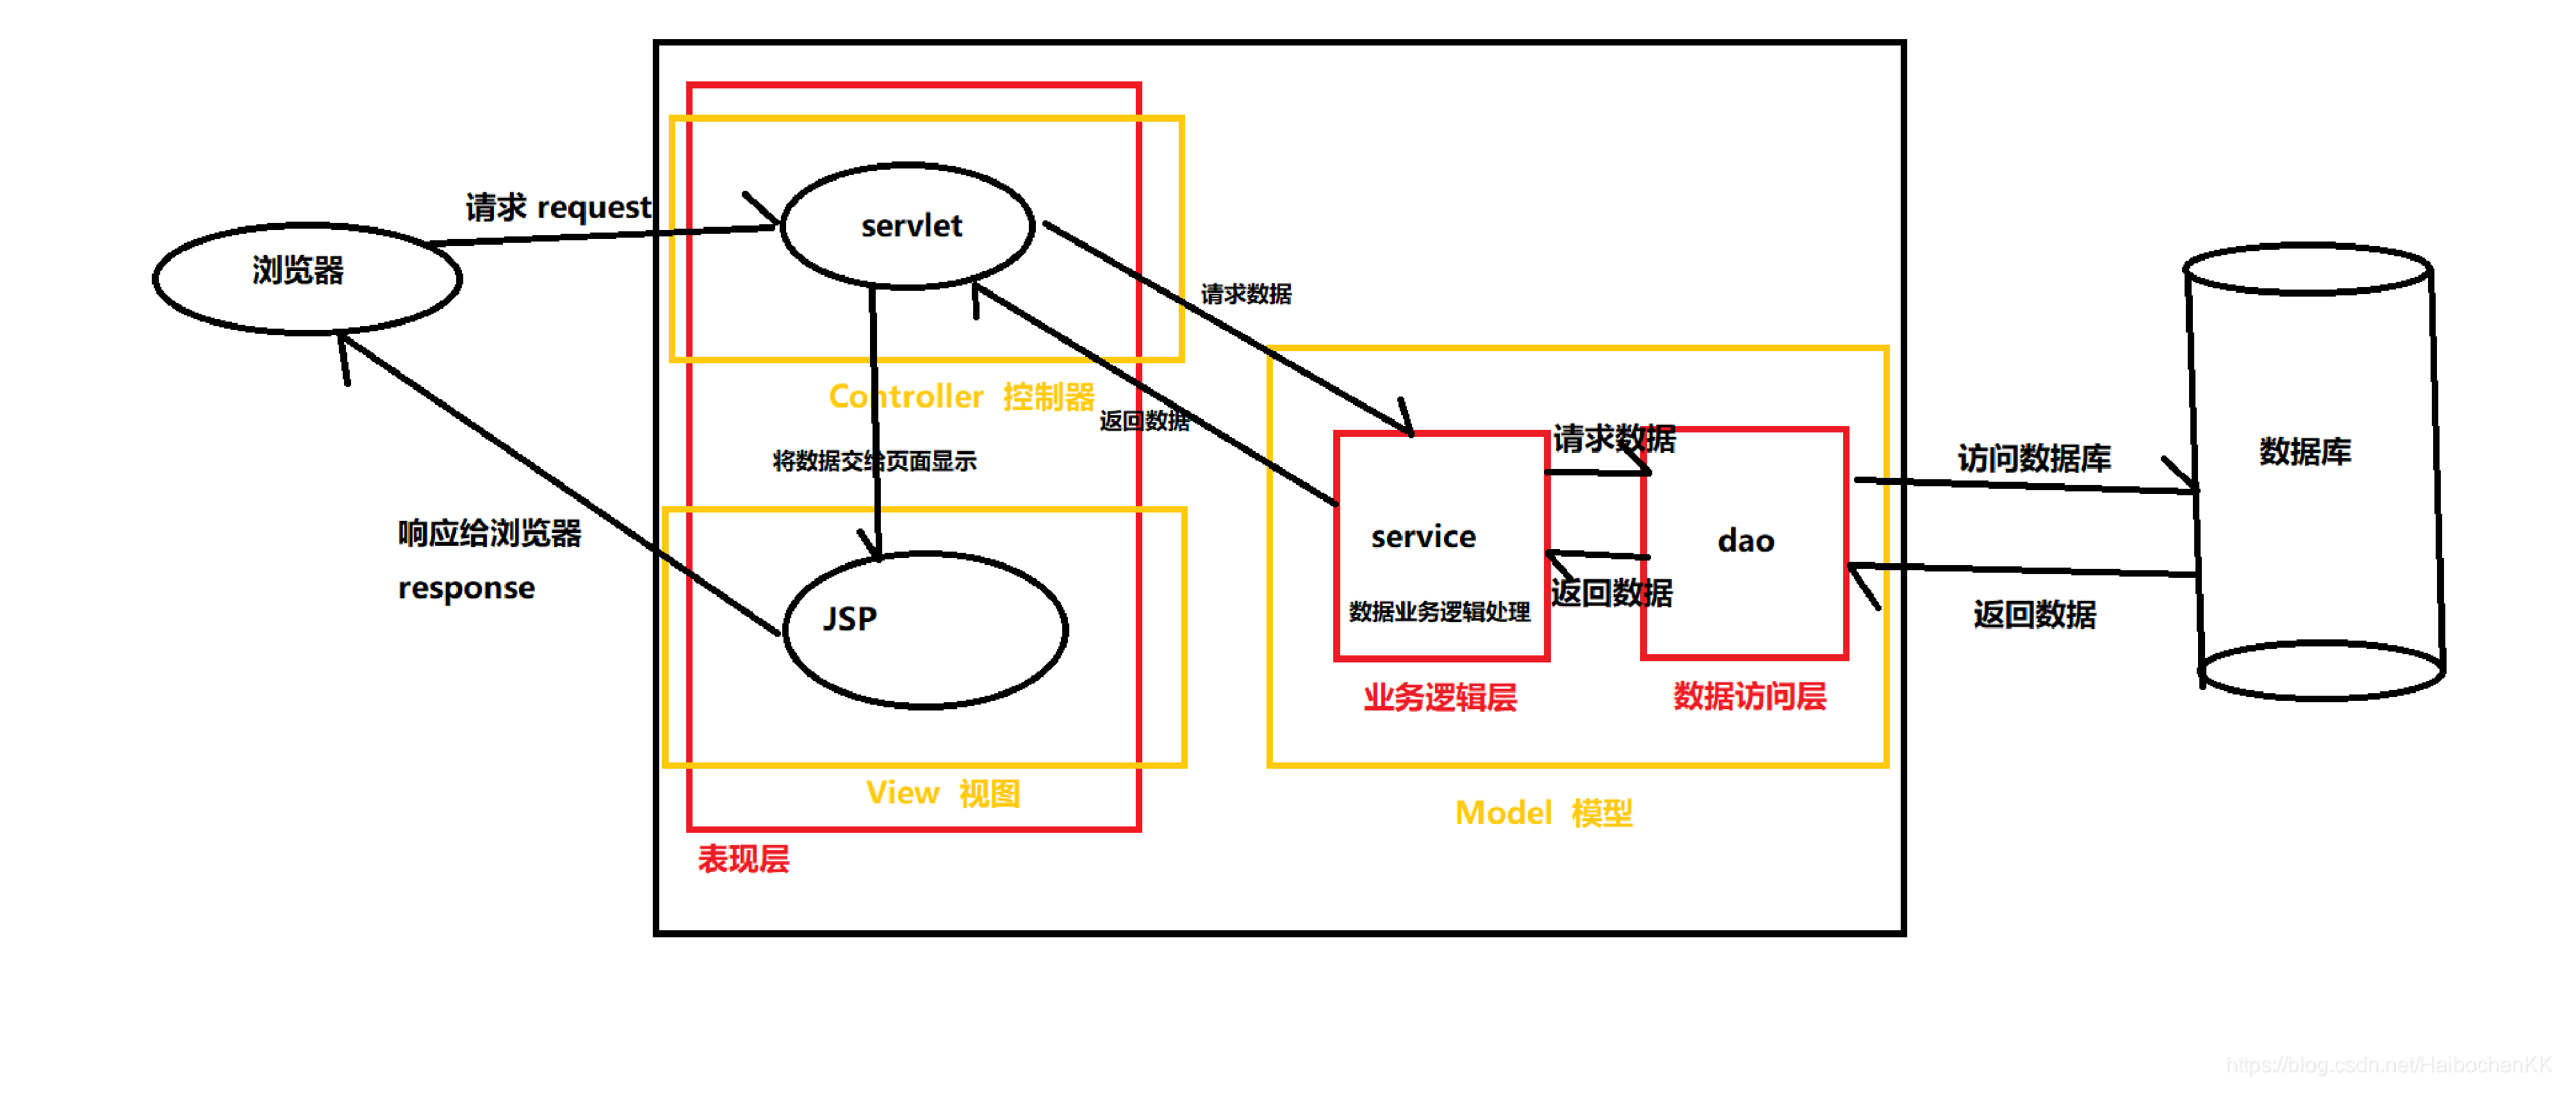
\includegraphics[width=6.2in]{figs/MVC.eps}
	\cnenfigcaption{模型-视图-控制器模式}{MVC pattern}
	\label{fig_1}
\end{figure}

MVC模式的设计初衷就是希望打破以往应用程序使用的大杂烩式的程序撰写方式,并间接诱使开发人员以更高的架构导向思维来思考应用程序的设计。MVC模式被广泛应用于各种软件开发框架和平台中,特别是在Web应用程序开发中。许多流行的Web框架,如Ruby on Rails、Spring MVC(Java框架)、Django(Python框架)等,都采用了MVC模式来组织和管理应用程序的代码结构。

\subsection{微服务(Mircroservices)}

微服务是以专注于单一职责与功能的小型功能区块为基础,利用模块化的方式组合出复杂的大型应用程序,各功能区块的使用与语言无关,而且复杂的服务背后是使用简单URI来开放接口,任何服务,任何细粒都能被开放。

微服务运用了以业务功能为中心的设计概念,应用程序在设计时就能先以业务功能或流程设计进行分割,将各个业务功能都独立实现成一个能自主执行的个体服务,然后再利用相同的协议将所有应用程序需要的服务组合起来,形成目标应用程序。若需要针对特定业务功能进行扩展,只要对实现该业务功能的微服务组件进行扩展即可,不需要整个应用程序都扩展。通过对高压力微服务组件(性能瓶颈)进行适当水平扩展,能增加计算资源利用率,实现“手术刀式”的系统优化。

在单体应用的时代,公共的业务功能经常没有明确的责任归属。最后要么各做各的,每个人都重新实现一遍;要么是随机一个人(一般是能力比较强或者比较热心的人)做到他负责的应用里面。在后者的情况下,这个人在负责自己应用之外,还要额外负责给别人提供这些公共的功能——而这个功能本来是无人负责的,仅仅因为他能力较强/比较热心,就莫名地背锅(这种情况还被美其名曰能者多劳)。结果最后大家都不愿意提供公共的功能。长此以往,团队里的人渐渐变得各自为政,不再关心全局的架构设计。通过设计合理的微服务组件可以解决该问题,从工程角度看,微服务架构模式使整个系统的分工更加明确,责任更加清晰。

\begin{figure}[H]
	\centering
	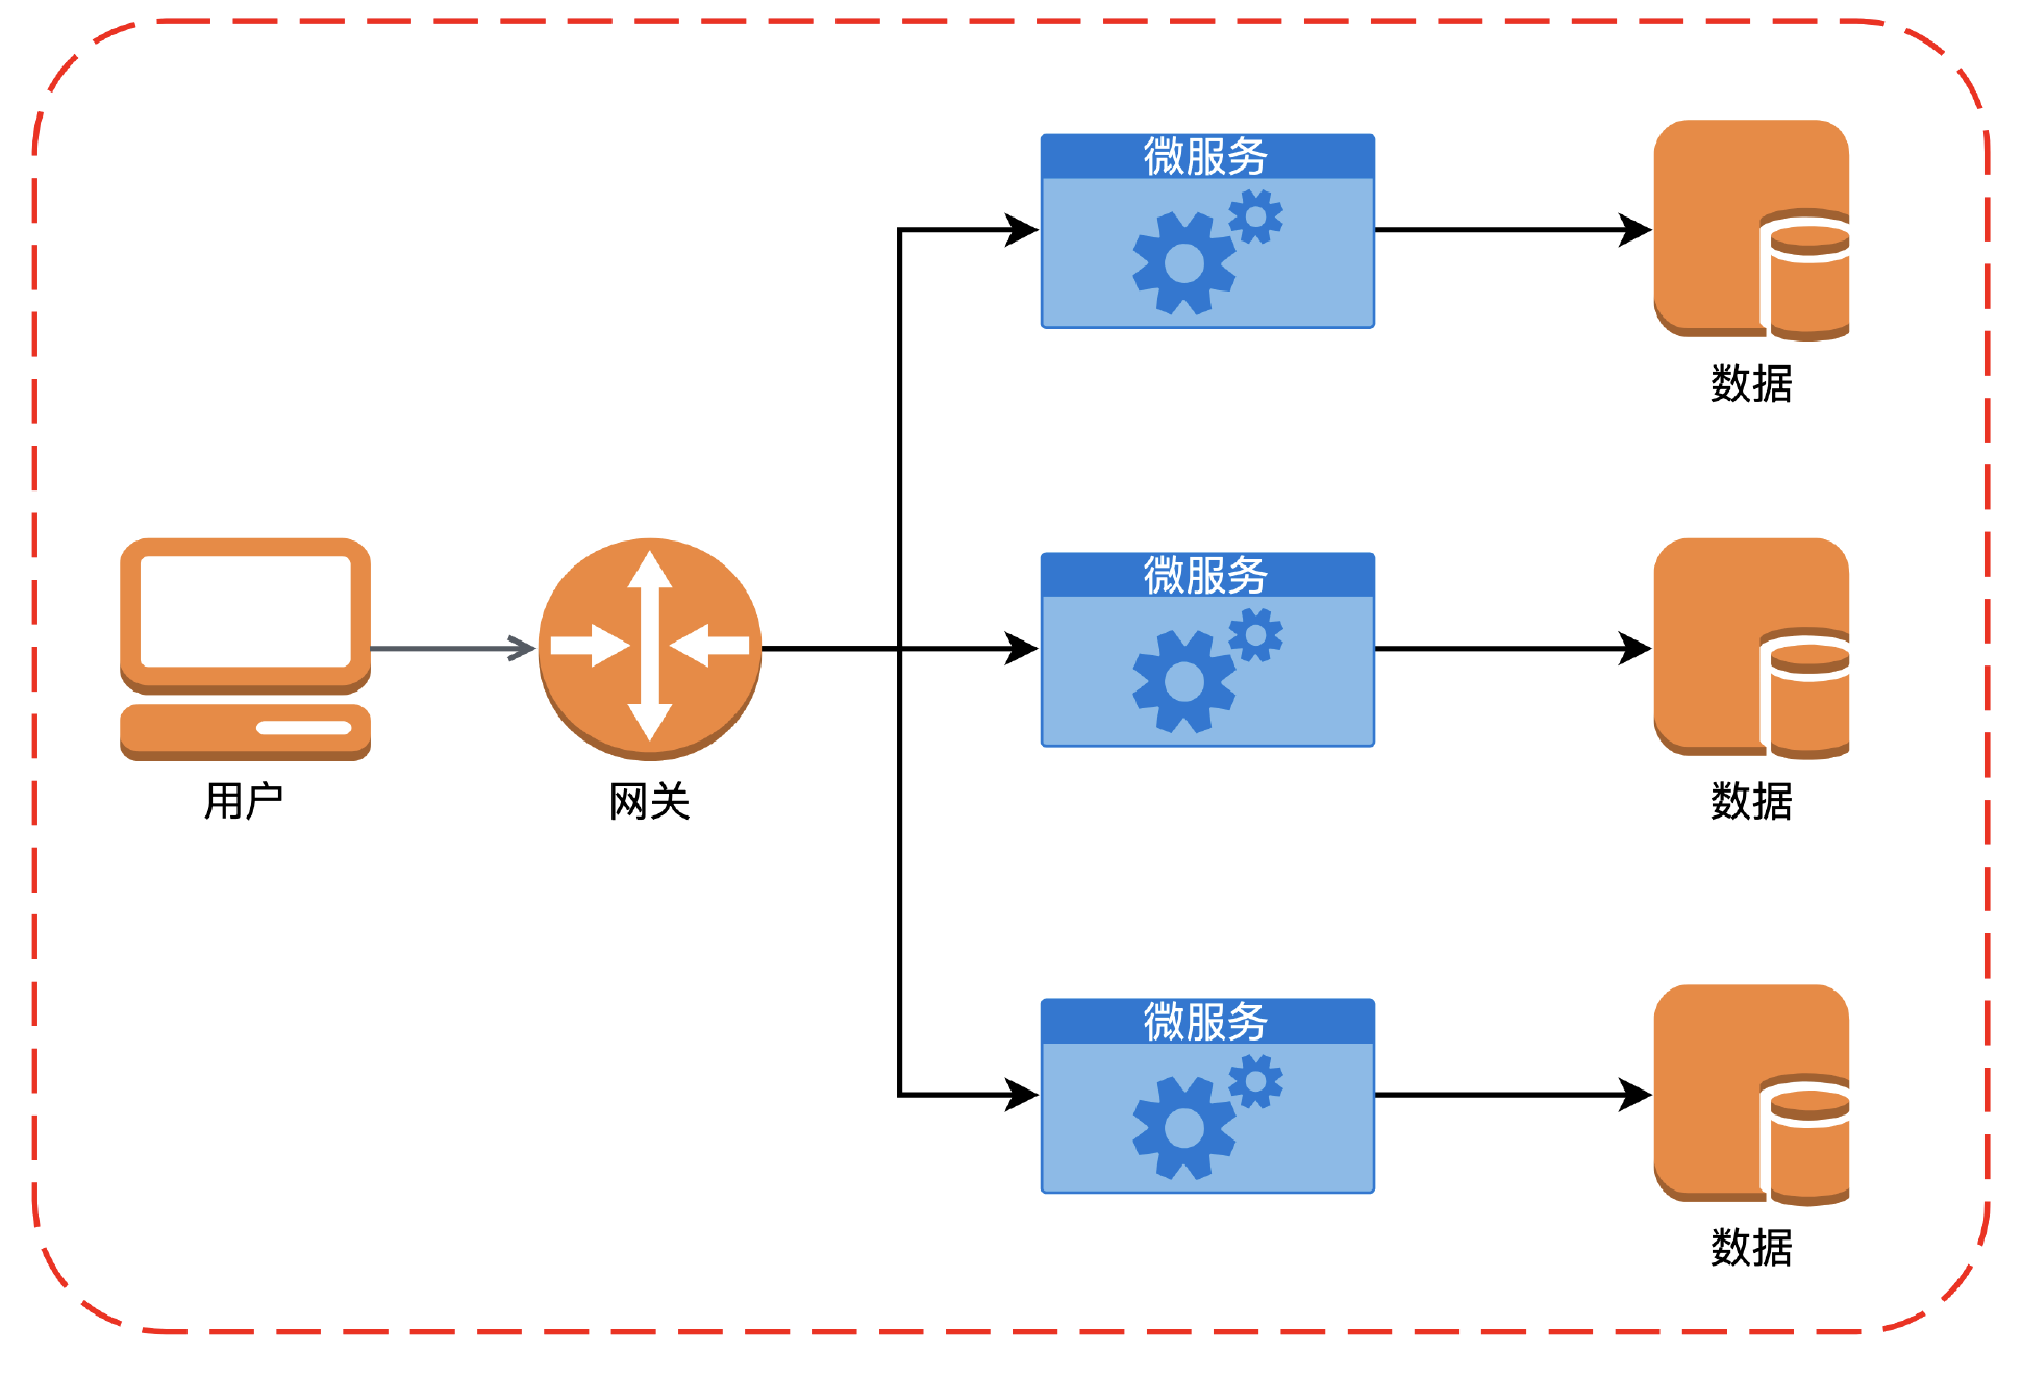
\includegraphics[width=6.2in]{figs/Micro.eps}
	\cnenfigcaption{微服务}{Mircroservices}
	\label{fig_1}
\end{figure}

\subsection{管道与过滤器模式(Pipes and Filters)}

管道-过滤器模式,把系统任务分成几个序贯的处理步骤。这些步骤,通过系统的数据流连接,一个步骤的输出,是下一个步骤的输入。管道过滤器模式的基本部件都有一套输入输出接口。每个部件从输入接口中读取数据,经过处理,将结果数据置于输出接口中,这样的部件称为“过滤器”。过滤器必须是独立的实体,不了解信息流从哪个过滤器流出,也不需要知道信息将流入哪个过滤器。可以指定输入的格式,可以确保输出的结果,但是可能不知道在管道之后将会是什么样子。过滤器之间,也不共享状态。因此通过使用管道过滤器模式,设计人员将整个系统的输入输出行为理解为单个过滤器行为的叠加与组合。这样可以将问题分解,化繁为简。同时通过使用新的过滤器替换旧的过滤器,软件系统可以很方便地进行维护和升级。

管道过滤器模式是面向数据流的软件体系结构。它最典型的应用是在编译系统中:一个普通的编译系统包括词法分析器,语法分析器,语义分析与中间代码生成器,优化器,目标代码生成器等一系列对源程序进行处理的过程。人们可以将编译系统看作一系列过滤器的连接体,按照管道过滤器模式进行设计。

\begin{figure}[H]
	\centering
	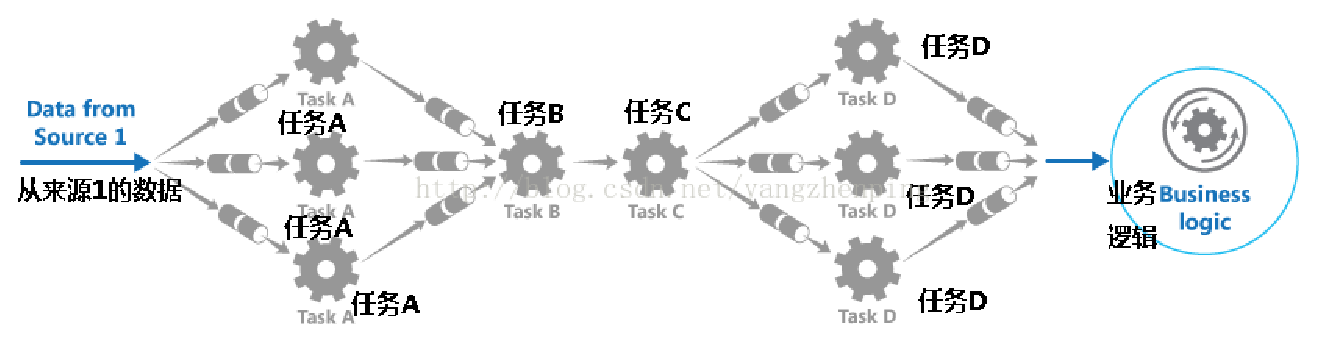
\includegraphics[width=6.2in]{figs/pipe.eps}
	\cnenfigcaption{负载平衡的管道过滤器模式}{Pipes and Filters(load balance)}
	\label{fig_1}
\end{figure}

当然管道过滤器模式由于其固化的模式,也存在一些缺点——较弱的交互式处理能力。管道过滤器模式不适合为与用户频繁交互的系统建模。在这种模式下,每个过滤器都有自己的数据,这些数据或者是从磁盘存储器中读取来,或者是由另一个过滤器的输出导入进来,整个系统没有一个共享的数据区。这样,当用户要操作某一项数据时,要涉及到多个过滤器对相应数据的操作,其实现较为复杂。

\subsection{事件驱动架构(Event Driven Architecture)}

事件驱动的架构是一种系统设计模式,以打造实时、敏捷的软件系统作为设计目标,其中系统的主要组件相互交互,通过事件和消息进行通信和协作。事件可以是用户的操作,也可以是来自其他组件的消息。通过将系统分解为一系列的独立组件,事件驱动的架构可以实现高度的模块化和可复用性。事件驱动的架构通常由以下几个主要组成部分构成:

\textcircled{1} 事件源:产生事件的组件,可以是用户界面、传感器、外部系统等。

\textcircled{2} 事件处理器:接收事件并进行处理的组件,可以是独立的模块或服务。

\textcircled{3} 事件通道:用于事件的传递和分发,可以是消息队列、发布/订阅系统等。

\textcircled{4} 事件消费者:从事件通道中获取事件并执行相应的操作。

事件驱动的架构的核心原理是异步通信和解耦。通过异步通信,将事件源与事件处理器解耦,实现了系统的解耦合或松耦合。同时,通过使用事件通道,可以实现事件的分发和多个消费者的并行处理。通过采用事件驱动架构,软件系统将变得像一个精心编排的交响乐队,每个组件都在自己的节拍上工作,共同创造出和谐而高效的软件交响曲。这种架构特别适合于构建那些需要快速响应、高度可扩展和灵活适应变化的系统。无论是在微服务架构、分布式系统还是实时数据处理领域,EDA都能展现其独特的魅力和力量。

\begin{figure}[H]
	\centering
	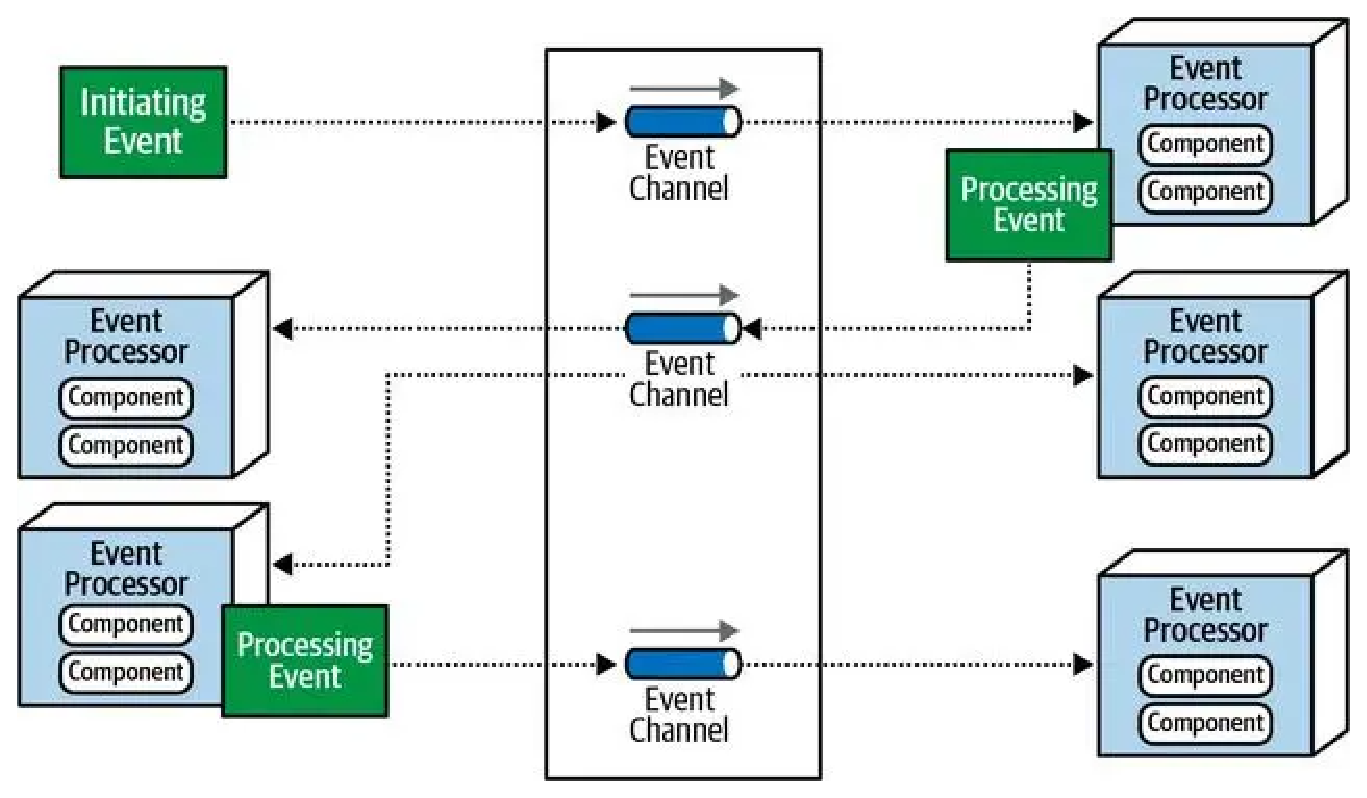
\includegraphics[width=6.2in]{figs/EDA.eps}
	\cnenfigcaption{事件驱动架构}{Event Driven Architecture}
	\label{fig_1}
\end{figure}

\section{软件体系结构的未来}

\textit{The software architecture of a system represents the design decisions related to overall system structure and behavior.}

\subsection{人工通用智能(AGI)}

目前,AGI(Artificial General Intelligence)是指具有广泛认知能力的人工智能,它是一种可以执行复杂任务的人工智能,能够完全模仿人类智能的行为。AGI可以被认为是人工智能的更高层次,它可以实现自我学习、自我改进、自我调整,进而解决任何问题而不需要人为干预。这与当前专门针对特定任务设计的人工智能(如聊天机器人,图像识别系统)有很大的区别。

\subsection{软件体系结构与AGI}

笔者认为AGI的思想实际上与软件体系结构出现的初衷是类似的。当前的软件架构,即使是最先进的云原生架构、微服务或AI集成系统,都是被设计用于处理特定的、定义良好的任务,而非理想意义上的,成为解决软件设计问题的普适方法。

软件架构设计能否使用AGI,甚至说,软件架构设计本身能否成为AGI,笔者认为将是决定软件架构设计发展上限的关键问题,也是软件架构发展的长期愿景。当前来看,二者之间存在着巨大鸿沟。但是我相信未来随着软件体系结构和人工智能的技术演进,软件架构的设计将集成更多的AI元素,提高自动化和智能化决策水平,同时克服伦理、安全和社会接受等多方面的挑战。

\section{总结}

作为控制软件复杂性、提高软件系统质量、支持软件开发和复用的重要手段之一,软件体系结构自提出以来,日益受到软件研究者和实践者的关注,并发展成为软件工程的一个重要的研究领域。本文是《软件体系结构》课程的课程总结,介绍了软件体系结构的定义、发展史以及包括分层系统、MVC、微服务在内的常见的软件架构模式。最后笔者结合AGI,指出软件架构设计可能的发展方向,探讨了软件体系结构领域未来的发展愿景。

在探索软件架构的演变过程中,我们见证了从单体架构到微服务架构,再到事件驱动架构的转变。这一变迁不仅是技术的升级,更是对高效、灵活和可持续发展的不懈追求。单体架构以其简洁性和直接性满足了早期软件开发的需求,随之出现的微服务架构,解决了单体架构在处理大型、复杂应用时的局限性。容器化技术,特别是Docker,为微服务提供了理想的运行和部署环境,同时保证了环境一致性和高效的资源利用。为更好地应对微服务组件间的协作需求,事件驱动架构应运而生。通过异步通信和松散耦合的方式,EDA增强了系统的弹性和可扩展性以及处理大量实时数据的能力,有助于实现高效的系统集成。

这一演变过程不仅仅是技术层面的变革,还伴随着组织结构和文化的转变。软件设计开发团队必须适应更加敏捷和协作的工作方式,培养持续学习和适应新技术的能力。

总的来说,软件体系结构的发展既是对过去技术的优化,也是对未来需求和挑战的预见。

\vfill

\begin{thebibliography}{99}
	
\bibitem{1} Software Architecture课程的课件. \url{https://njuics.github.io/sa2024/1}. (2024)

\bibitem{2} Software Architecture. \url{https://www.sei.cmu.edu/our-work/software-architecture/}

\bibitem{3} Perry, Dewayne \& Wolf, Alexander. (2000). Foundations for the Study of Software Architecture. ACM SIGSOFT Software Engineering Notes. 17. 10.1145/141874.141884. 

\bibitem{4} 孙昌爱,金茂忠,刘超.软件体系结构研究综述[J].软件学报,2002(07):1228-1237.

\bibitem{5} 梅宏,申峻嵘.软件体系结构研究进展[J].软件学报,2006(06):1257-1275.

\end{thebibliography}

\newpage

\makeentitle

\end{document}
